\documentclass[letterpaper, 12pt]{amsart}

\usepackage{amssymb}
\usepackage{amsthm}
\usepackage[letterpaper, margin=1.25in]{geometry}
\usepackage{tikz}

\title{Path Coloring Algorithms on Planar Graphs}
\author{Aven Bross}

\theoremstyle{definition}
\newtheorem{definition}{Definition}[section]

\theoremstyle{definition}
\newtheorem{example}{Example}[section]

\theoremstyle{thm}
\newtheorem{theorem}{Theorem}[section]

\theoremstyle{definition}
\newtheorem{algorithm}{Algorithm}[section]


\tikzset{%
    every node/.style={circle, fill, draw, minimum size=1mm, scale=.4}
}


\begin{document}

\maketitle

\section{Planar Graphs}

A \textit{(simple) graph} $G(V,E)$ consists of a finite set $V$ of
\textit{vertices} and a set $E$ of two element subsets of $V$ known as
\textit{edges}. We will often refer to the graph as $G$ and the vertex and
edge sets as $V(G)$ and $E(G)$ respectively. As shortand we will denote an edge
$\{u,v\}\in E(G)$ simply as $uv$.

Two vertices $u,v\in V(G)$ are \textit{adjacent}
if $uv\in E(G)$. Vertices $u$ and $v$ are known as the \textit{endpoints}
of $uv$. The  vertices adjacent to $v\in V(G)$ are known as the 
\textit{neighbors} of $v$. The number of neighbors is known as the
\textit{degree} of $v$, denoted $\text{deg}(v)$.

A graph $G'$ is a \textit{subgraph} of $G$ if $V(G')\subseteq V(G)$ and
$E(G')\subseteq E(G)$. If $S\subseteq V(G)$ the \textit{induced subgraph} of $S$
on $G$ is the graph with vertex set $S$ and edge set $\{uv\in E(G)|u,v\in S\}$.
Equivalently we say a subgraph $G'$ is \textit{induced} if there are no edges
from $G$ that may be added without adding vertices to $G'$.

A complete graph $K_n$ consists of $n$ vertices and all possible edges.
A length $n$ path consists of vertices $v_1,v_2,\ldots,v_n$ and edges $v_1v_2,
v_2v_3,\ldots,v_{n-1}v_n$. A length $n$ cycle, or $n$-cycle, consists of a
length $n$ path and the additional edge $v_1v_n$. We will often denote a path
or cycle $G$ by simply listing its vertices in order, i.e. $G=v_1v_2\ldots v_n$.

\begin{figure}
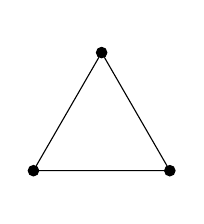
\begin{tikzpicture}
	\node (a) at (0cm,0.75cm) {};
	\node (b) at (0.866cm,-0.75cm) {};
	\node (c) at (-0.866cm,-0.75cm) {};
	\node [draw=none, fill=none] (1) at (0cm,-1cm) {};
	\node [draw=none, fill=none] (2) at (0cm,1cm) {};
	\draw (a) -- (b) -- (c) -- (a);
\end{tikzpicture}
$\qquad$
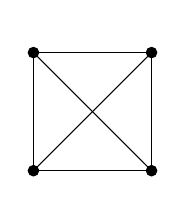
\begin{tikzpicture}
	\node (a) at (0.75cm,0.75cm) {};
	\node (b) at (0.75cm,-0.75cm) {};
	\node (c) at (-0.75cm,-0.75cm) {};
	\node (d) at (-0.75cm,0.75cm) {};
	\node [draw=none, fill=none] (1) at (0cm,-1cm) {};
	\node [draw=none, fill=none] (2) at (0cm,1cm) {};
	\draw (a) -- (b) -- (c) -- (d) -- (a);
	\draw (a) -- (c); \draw (b) -- (d);
\end{tikzpicture}
$\qquad$
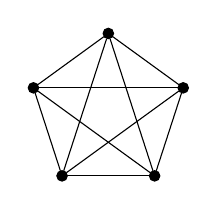
\begin{tikzpicture}
	\node (a) at (90:1cm) {};
	\node (b) at (162:1cm) {};
	\node (c) at (234:1cm) {};
	\node (d) at (306:1cm) {};
	\node (e) at (18:1cm) {};
	\node [draw=none, fill=none] (1) at (0cm,-1cm) {};
	\node [draw=none, fill=none] (2) at (0cm,1cm) {};
	\draw (a) -- (b); \draw (a) -- (c); \draw (a) -- (d); \draw (a) -- (e);
	\draw (b) -- (c); \draw (b) -- (d); \draw (b) -- (e); \draw (c) -- (d);
	\draw (c) -- (e); \draw (d) -- (e);
\end{tikzpicture}
$\qquad$
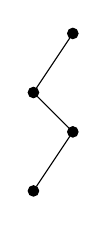
\begin{tikzpicture}
	\node (a) at (0.25cm,1cm) {};
	\node (b) at (-0.25cm,0.25cm) {};
	\node (c) at (0.25cm,-0.25cm) {};
	\node (d) at (-0.25cm,-1cm) {};
	\draw (a) -- (b) -- (c) -- (d);
\end{tikzpicture}
$\qquad$
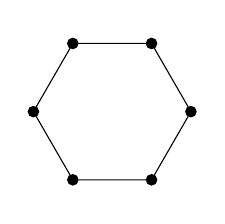
\begin{tikzpicture}
	\node (a) at (180:1cm) {};
	\node (b) at (120:1cm) {};
	\node (c) at (60:1cm) {};
	\node (d) at (0:1cm) {};
	\node (e) at (300:1cm) {};
	\node (f) at (240:1cm) {};
	\node [draw=none, fill=none] (1) at (0cm,-1cm) {};
	\node [draw=none, fill=none] (2) at (0cm,1cm) {};
	\draw (a) -- (b) -- (c) -- (d) -- (e) -- (f) -- (a);
\end{tikzpicture}

\caption{Drawings of $K_3$, $K_4$, $K_5$, a length $4$ path, and a
	$5$-cycle.}
\end{figure}

A \textit{drawing} of a graph $G$ maps each vertex of $G$ to a point in the plane
and each edge to a curve connecting its endpoints.
A \textit{planar embedding} is a drawing of $G$ where
edge curves intersect only at their endpoints. We say a graph is \textit{planar}
if it admits a planar embedding. A planar graph together with a planar embedding
is a \textit{plane graph}. In a plane graph we shall assume all edge curves are
line segments, which is allowable due to the following result by F\'ary.

\begin{theorem}[F\'ary]
Every planar graph admits a planar embedding in which each edge curve is a line
segment.
\end{theorem}

\begin{figure}
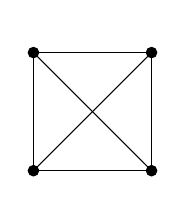
\begin{tikzpicture}
	\node (a) at (0.75cm,0.75cm) {};
	\node (b) at (0.75cm,-0.75cm) {};
	\node (c) at (-0.75cm,-0.75cm) {};
	\node (d) at (-0.75cm,0.75cm) {};
	\node [draw=none, fill=none] (1) at (0cm,-1cm) {};
	\node [draw=none, fill=none] (2) at (0cm,1cm) {};
	\draw (a) -- (b) -- (c) -- (d) -- (a);
	\draw (a) -- (c); \draw (b) -- (d);
\end{tikzpicture}
$\qquad$
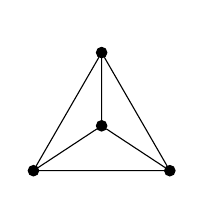
\begin{tikzpicture}
	\node (a) at (0cm,0.75cm) {};
	\node (b) at (0.866cm,-0.75cm) {};
	\node (c) at (-0.866cm,-0.75cm) {};
	\node (d) at (0cm, -0.18cm) {};
	\node [draw=none, fill=none] (1) at (0cm,-1cm) {};
	\node [draw=none, fill=none] (2) at (0cm,1cm) {};
	\draw (a) -- (b) -- (c) -- (d) -- (a);
	\draw (a) -- (c); \draw (b) -- (d);
\end{tikzpicture}

\caption{A nonplanar drawing and a planar embedding of $K_4$.}
\end{figure}

Let $G$ be a plane graph. A \textit{face} of $G$ is a maximal region
of the plane not containing any point used in the embedding.
The unbounded face is known as the \textit{outer face}.
We will always refer to a face by the subgraph of
vertices and edges that lie on its border. For brevity, we have
not fully formalized the definitions of curve, region, or border. However, these
definitions are fairly standard and may be found in many graph theory texts, for
example \cite{west}.

A planar graph is said to be \textit{triangulated} if adding any new edge
results in a nonplanar graph. A face is said to be a \textit{triangle} if it is
a $3$-cycle. It is easy to see that all faces in a triangulated
plane graph are triangles: if any face has more than three vertices then we may
add an edge curve connecting two face vertices without crossing existing edges.
If a plane graph has a cycle for its outer face and triangles for all other
faces it is said to be \textit{weakly triangulated}.

A \textit{rotation scheme} for a graph $G$ is a cyclic ordering of the incident
edges of each $v\in V(G)$. Planar embeddings naturally induce a rotation
scheme by the position of edge curves around each vertex. In fact, with respect
algorithms, the induced rotation scheme is the
most useful property of an embedding. Rotation schemes provide a means of
orienting ourselves within a graph, while points and lines in Euclidean space
simply add unnecessary complexity. Therefore, while we may often visualize plane
graphs with drawings, embeddings will always be represented solely by their
induced rotation scheme. One may note that if we consider two embeddings of a
graph $G$ equivalent if they induce the same rotation scheme, we form an
equivalence relation on the planar embeddings of $G$.

\section{Representations and Time Complexity}

The basic operation for all time complexity discussions shall be
performing a single array lookup or a single comparison between integral type
variables. Vertices shall be represented by integers and vertex properties will
be stored in arrays indexed by vertices. Each vertex property will either
be an integer, a pair of integers, or an array of integers. Therefore accessing
or comparing vertex properties shall, in general, be $\mathcal{O}(1)$ time.

Suppose $G$ is a plane graph. We will always denote number of vertices in $G$
with $n$ and the number of edges with $m$. Also, from now on we assume
$V(G)=\{1,2,\ldots,n\}$. By Euler's formula $m\le 3n-6$ and therefore, with
respect to time complexity, $\mathcal{O}(m)=\mathcal{O}(n)$. For compatibility
with mathematical notation, arrays indices will always start at $1$. If $A$ is
an array and $i$ a positive integer we shall denote element $i$ of $A$ with
square brackets, $A[i]$.


For each $v\in V(G)$ we define an array called an
\emph{adjacency list} containing the neighbors of $v$ ordered according to
the rotation scheme of the embedding. The full plane graph $G$ is then
represented by a size $n$ array $A$ of adjacency lists, indexed by vertices.
That is, for $v\in V(G)$, $A[v]$ is the adjacency list for $v$. In many cases we
will wish for the ability find a vertex $u$ in $v$'s adjacency list simply from
$v$'s entry in $u$'s adjacency list. To allow this in $\mathcal{O}(1)$ time we
shall also define an array $I[v]$ called an \emph{index list} for each vertex
$v$. For each $i\in\{1,2,\ldots,\text{deg}(v)\}$, let $u=A[v][i]$ and let $j$ be
the index such that $A[u][j]=v$. We then define $I[v][i]=j$. The array $I$
containing index lists for each vertex may be constructed in $\mathcal{O}(m)$
time from $A$.

\section{A Brief History of Coloring}

A $k$\textit{-coloring} of a graph assigns each vertex one of $k$ possible
colors. Equivalently, a $k$-coloring partitions the vertices of a graph into $k$
disjoint sets called \textit{color classes}. A \textit{path $k$-coloring} is
a $k$-coloring such that the induced subgraph of each color class consists of
one or more disjoint paths. Poh \cite{poh} showed the following procedure for
path $3$-coloring triangulated plane graphs.

A coloring is \textit{proper} if no pair of adjacent vertices recieve the same
color, equivalently, the color classes each consist of nonadjacent vertices. It
is clear not all planar graphs admit a proper $3$-coloring since $K_4$ is planar
and requires $4$ colors. Whether all planar graphs may be properly colored with
$4$ colors remained one of the premier open questions in graph theory until it
was shown to be true by Appel and Haken in 1976 \cite{appelhaken1, appelhaken2}.

A \textit{$l$-defective} $k$-coloring

\begin{theorem}[Poh]
Let $G$ be a weakly triangulated plane graph with outer face $C$ that has
been $2$-colored such that each color class induces a non-empty path. This
$2$-coloring may then be extended to a path $3$-coloring of $G$ such that no
vertex in $V(C)$ recieves a same color neighbor in $V(G)\setminus V(C)$.
\end{theorem}

\begin{proof}
If $|V(G)|\le 3$ there are no vertices to color. Let $|V(G)|>3$ and
suppose the theorem holds for all graphs $H$ with $|V(H)|<|V(G)|$. Let
$P=p_0\ldots p_n$ and $Q=q_0\ldots q_m$ denote the two induced paths from the
$2$-coloring of $C$, ordered such that the edges $p_0q_0$ and $p_nq_m$ are in
$C$. Suppose there exist uncolored vertices, that is $V(G)\setminus V(C)\ne
\emptyset$.

Let $t_0$ be the vertex forming a face with $p_0$ and $q_0$. If
$t_0\in P$, this face is already colored and we consider the graph bounded by
$P-p_0$ and $Q$. Similarly, if $t_0\in Q$ then the inductive hypothesis applies
to the graph bounded by $P$ and $Q-q_0$. Let $t_1$ be the vertex forming a face
with $p_n$ and $q_m$ and proceed in the same manner until $t_1$ is not in either
path.

Suppose there exists an induced path $T$ from $t_0$ to $t_1$. We color
$T$ the remaining color not assigned to $P$ or $Q$ and apply the inductive
hypothesis to the subgraph bounded by $P$ and $T$, and the subgraph bounded by
$T$ and $Q$. With only the path $T$ in common between the two subgraphs, the
combined $3$-coloring forms a path coloring of $G$.

Suppose no such path exists from $t_0$ to $t_1$. Since $G$ is weakly
triangulated there must exist an edge $p_iq_j\in E(G)\setminus E(C)$ with
$p_i\in P$ and $q_j\in Q$. We separately apply the inductive hypothesis to the
subgraph bounded by $p_0\ldots p_i$ and $q_0\ldots q_j$, and the subgraph
bounded by $p_i\ldots p_n$ and $q_j\ldots q_m$. The two subgraphs only share the
vertices $p_i$ and $q_j$, thus the combined $3$-coloring forms a path coloring
of $G$.
\end{proof}

\section{Path 3-List-Coloring}


\begin{thebibliography}{2}  % "2" because there are two references
\bibitem{west}
	D. West (2001).
	\textit{Introduction to Graph Theory},
	2nd ed., Pearson.
\end{thebibliography}
\end{document}
